\documentclass[11pt]{amsart}
\usepackage[margin=1.15in]{geometry}
\usepackage[T1]{fontenc}
\usepackage{lmodern}
\usepackage{amssymb,amsmath,mathtools}
\usepackage{graphicx,float}
\usepackage[hidelinks]{hyperref}
\usepackage[expansion=false]{microtype}

\newtheorem{theorem}{Theorem}[section]
\newtheorem{proposition}[theorem]{Proposition}
\newtheorem{lemma}[theorem]{Lemma}
\newtheorem{corollary}[theorem]{Corollary}
\newtheorem{mainthm}{Theorem}
\renewcommand{\themainthm}{\Alph{mainthm}}
\theoremstyle{definition}
\newtheorem{definition}[theorem]{Definition}
\newtheorem{remark}[theorem]{Remark}

\newcommand{\RR}{\mathbb{R}}
\newcommand{\ZZ}{\mathbb{Z}}
\newcommand{\dd}{\,\mathrm{d}}
\DeclareMathOperator{\arcsinh}{arcsinh}
\DeclareMathOperator{\arccosh}{arccosh}
\newcommand{\Dslash}{D\!\!\!\!/\,}

\setlength{\emergencystretch}{2.5em}
\hbadness=2000
\raggedbottom
\begin{document}

\title[The negative prolate spectrum]{The Negative Prolate Spectrum\\ and the Riemann--Siegel Theta Function}

\author{Deep Bhattacharjee}
\address{Formerly, Electro-Gravitational Space Propulsion Laboratory (EGSPL), Bhubaneswar, Odisha 751030, India}
\address{Formerly, University of Calcutta (Heramba Chandra College), 23/49 Gariahat Road, Golpark, Kolkata 700029, West Bengal, India}
\email{d.bhattacharjee@erl-forschung.de}
\email{itsdeep@live.com}
\email{egspl@proton.me (GitHub-related contact; GitHub account creelie)}
\urladdr{https://orcid.org/0000-0003-0466-750X}

\begin{abstract}
Connes and Moscovici found that the negative eigenvalues of the self-adjoint prolate wave operator reproduce the growth of the zeros of the Riemann zeta function. In the published version, their counting law for the associated Dirac operator contains a term $-(\log E)/2\pi$. We prove that this term is absent. The proof is an elementary phase analysis, and it places the eigenvalues, up to $O(t^{-2/3})$, at the points where the Riemann--Siegel theta function equals $(n-\tfrac38)\pi$.

\medskip\noindent\textbf{Keywords:} prolate wave operator; Pr\"ufer angle; Riemann zeta function.

\smallskip\noindent\textbf{MSC 2020:} 34L20 (primary); 34B24, 11M06.
\end{abstract}

\maketitle

\section{Introduction}\label{sec:intro}

For $\lambda>0$ the prolate wave operator is the differential expression
\begin{equation}\label{eq:W}
(W\xi)(x)=-\frac{\dd}{\dd x}\Big((\lambda^2-x^2)\frac{\dd\xi}{\dd x}\Big)+(2\pi\lambda x)^2\,\xi(x),\qquad x\in\RR .
\end{equation}
On the interval $[-\lambda,\lambda]$ it commutes with time and band limiting, which is the observation of Slepian and Pollak behind the prolate spheroidal wave functions \cite{SP61}. Connes and Moscovici studied $W$ on the whole line \cite{CM21,CM22}. They showed that $W$ has a unique self-adjoint extension $W_{\rm sa}$ in $L^2(\RR)$ that commutes with the projection $P_\lambda$ onto functions supported in $[-\lambda,\lambda]$ and with its Fourier conjugate. The spectrum of $W_{\rm sa}$ is discrete and unbounded in both directions. The positive part on $[-\lambda,\lambda]$ is the classical prolate spectrum. The negative eigenvalues live outside the interval, their eigenfunctions lie in the Sonin space, and their growth matches that of the squares of the zeros of $\zeta(\tfrac12+it)$. This last point ties the operator to the positivity of Weil's functional at the archimedean place \cite{CC21}.

For $\lambda=\sqrt2$, Connes and Moscovici built a Dirac-type square root $2\Dslash$ of the even part of $W_{\rm sa}$ outside the interval, using a Darboux factorisation. Its imaginary eigenvalues are $\pm 2\sqrt{\mu}$, where $\mu$ runs over the negative eigenvalues. Let $N(E)$ be the number of these eigenvalues with imaginary part in $(0,E]$. The preprint \cite[Thm.~6.1]{CM21} states
\begin{equation}\label{eq:arxiv}
N(E)=\frac{E}{2\pi}\Big(\log\frac{E}{2\pi}-1\Big)+O(1),
\end{equation}
which is the smooth part of the Riemann--von Mangoldt formula. Its proof, however, rests on a semiclassical phase-space count \cite[Prop.~4.2]{CM21} that is not a proof about eigenvalues. The published version \cite[Thm.~5.1, Eq.~(33)]{CM22} instead asserts
\begin{equation}\label{eq:pnas}
N(E)=\frac{E}{2\pi}\Big(\log\frac{E}{2\pi}-1\Big)-\frac{\log E}{2\pi}+O(1),
\end{equation}
and derives it from Heywood's formula \cite{Hey54} and later extensions of it, applied after a Liouville transformation. The extra term would push the spectrum away from the zeros by an unbounded amount, against the paper's own figures.

Formula \eqref{eq:pnas} is false. The hypotheses of Heywood's formula fail, as also observed in \cite{TWW26}, at the endpoint $x=\lambda$, where the reduced potential has the critical singularity $-1/(4t^2)$. There the correct contribution is a fixed Bessel phase $\pi/4$, not a logarithmically growing term. We prove the law \eqref{eq:arxiv} for every $\lambda>0$ and both parities, with a quantisation rule for the individual eigenvalues. Write
\begin{equation}\label{eq:kappa}
\kappa=2\pi\lambda^2,\qquad \Phi(E)=E\log\frac{4E}{\kappa}-E+\frac{\pi}{4}.
\end{equation}

\begin{mainthm}\label{thm:A}
Let $W_{\rm sa}^{+}$ and $W_{\rm sa}^{-}$ be the restrictions of $W_{\rm sa}$ to even and to odd functions. There is a continuous, strictly increasing function $\Theta:[0,\infty)\to\RR$ with
\[
\Theta(E)=\Phi(E)+O\big(E^{-2/3}\big)\qquad(E\to\infty)
\]
such that, for $E>0$, the number $-E^2$ is an eigenvalue of $W_{\rm sa}^{+}$ exactly when $\Theta(E)\in\pi\ZZ$, and of $W_{\rm sa}^{-}$ exactly when $\Theta(E)\in\frac{\pi}{2}+\pi\ZZ$. All these eigenvalues are simple. Consequently the number $N_\pm(E)$ of eigenvalues of $W_{\rm sa}^{\pm}$ in $[-E^2,0)$ satisfies
\[
N_\pm(E)=\frac{E}{\pi}\Big(\log\frac{2E}{\pi\lambda^2}-1\Big)+O(1),
\]
and there are integers $n_\pm$ such that the eigenvalues $-(E_n^\pm)^2$, listed with $E_1^\pm<E_2^\pm<\cdots$, satisfy
\[
E_n^{\pm}\log\frac{2E_n^\pm}{\pi\lambda^2}-E_n^\pm=\Big(n+n_\pm\mp\frac14\Big)\pi+O\big((E_n^\pm)^{-2/3}\big).
\]
\end{mainthm}

Thus the even and the odd negative eigenvalues interlace, and both are governed by a single phase function. Figure~\ref{fig:levels} shows the levels.

\begin{figure}[H]
\centering
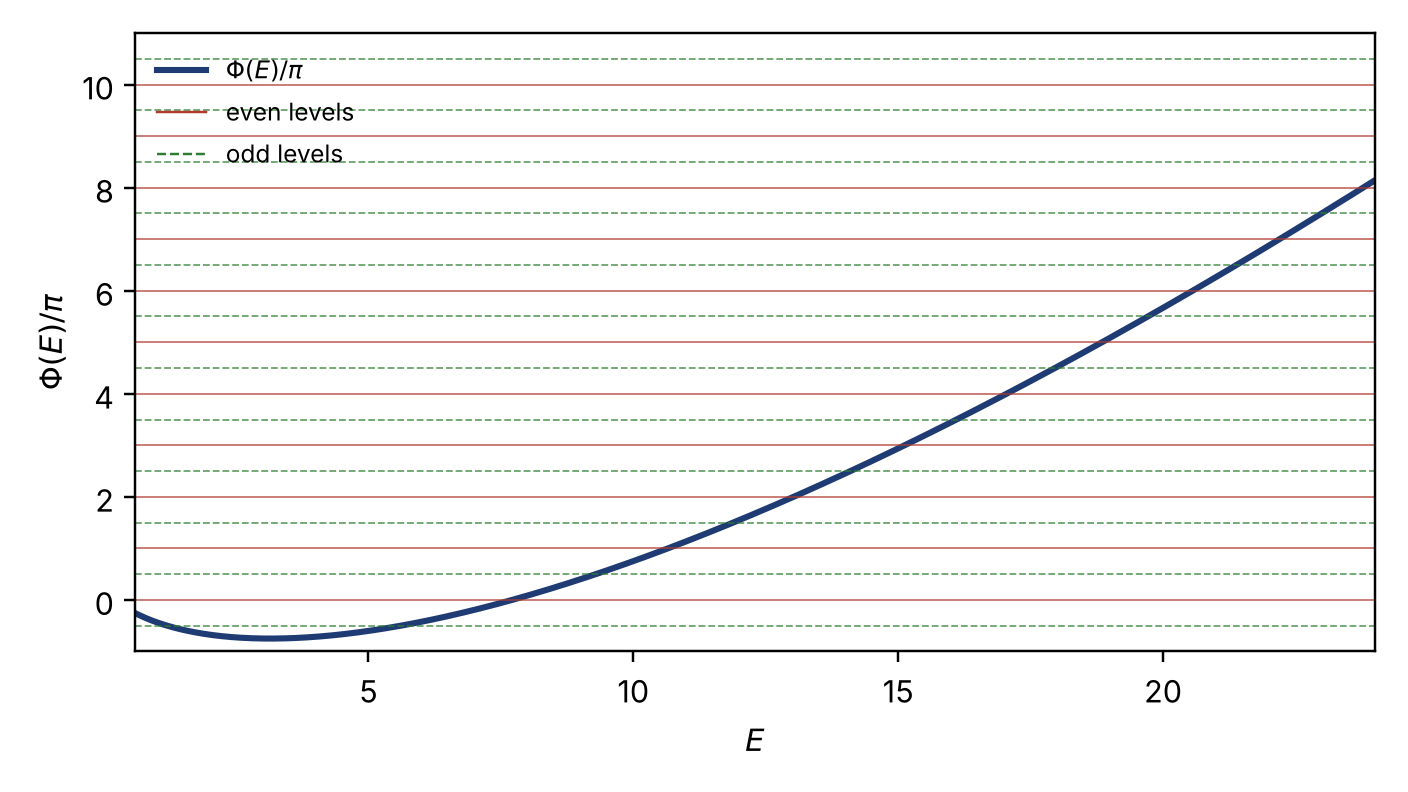
\includegraphics[width=0.78\textwidth]{fig_levels.png}
\caption{The function $\Phi(E)/\pi$ for $\lambda=\sqrt2$. Up to $O(E^{-2/3})$, even negative eigenvalues $-E^2$ occur where it meets an integer, odd ones where it meets a half-integer.}
\label{fig:levels}
\end{figure}

For $\lambda=\sqrt2$ the phase $\Phi$ turns out to be a shifted copy of the Riemann--Siegel theta function
\[
\vartheta(t)=\arg\Gamma\Big(\frac14+\frac{it}{2}\Big)-\frac{t}{2}\log\pi=\frac t2\log\frac{t}{2\pi}-\frac t2-\frac{\pi}{8}+O\Big(\frac1t\Big).
\]

\begin{mainthm}\label{thm:B}
Let $\lambda=\sqrt2$ and let $0<t_1<t_2<\cdots$ be the positive imaginary parts of the eigenvalues of $2\Dslash$. There is an integer $n_0$ with
\[
\vartheta(t_n)=\Big(n+n_0-\frac38\Big)\pi+O\big(t_n^{-2/3}\big).
\]
The counting function satisfies $N(E)=\vartheta(E)/\pi+O(1)$, so \eqref{eq:arxiv} holds and \eqref{eq:pnas} does not. Moreover
\[
N(T)-N_\zeta(T)=-S(T)+O(1),
\]
where $N_\zeta(T)$ counts the zeros of $\zeta(s)$ with $0<\Im s\le T$ and $S(T)=\pi^{-1}\arg\zeta(\frac12+iT)$. In particular $N(T)-N_\zeta(T)$ is unbounded above and below.
\end{mainthm}

The points $\vartheta(t)=m\pi$ are the Gram points. Theorem~\ref{thm:B} says that the Connes--Moscovici spectrum sits, asymptotically, on the lattice $\vartheta\equiv-\tfrac38\pi$ modulo $\pi$, a rigid version of Gram's law. The zeros follow the same lattice on average, $N_\zeta(T)=\vartheta(T)/\pi+1+S(T)$, but they fluctuate around it by $S(T)$, and the operator does not see this fluctuation.

\subsection*{Relation to other work}
Ramis, Richard-Jung and Thomann proved that the eigenvalues of $W_{\rm sa}$ not coming from the interval problem are negative, and they characterised them through spectral determinants \cite{RRT25}. Taira, Willems and Wrochna have recently obtained the logarithmic Weyl law and a Bohr--Sommerfeld rule for $W_{\rm sa}$ by microlocal methods \cite{TWW26}, for every value of the parameter \cite[Remark~1.4]{TWW26}. They point out that classical Sturm--Liouville asymptotics such as Heywood's do not apply at the degenerate endpoints. Their quantisation rule is stated in terms of a renormalised action integral, and its remainder is sharper than ours; their Weyl law already rules out \eqref{eq:pnas}, although the consequence for the Dirac counting function is not drawn there. The present argument is different and short. It uses only a Pr\"ufer angle, a comparison with the Bessel function $J_0$ at the singular endpoint, and an integration by parts at infinity. What is new here is the closed form of the phase in terms of $\vartheta$, the resulting Gram-type rule and the comparison $N-N_\zeta=-S+O(1)$, and the explanation of where the term in \eqref{eq:pnas} comes from. This note continues the author's interest in operator-theoretic and noncommutative structures \cite{Bha22a,Bha22b,BSN26}.

\section{The outer problem}\label{sec:outer}

Throughout, $\lambda>0$ is fixed and $\kappa=2\pi\lambda^2$. We use the description of the domain of $W_{\rm sa}$ given in \cite[\S2]{CM21}. A function $\xi$ in the maximal domain belongs to the domain of $W_{\rm sa}$ if and only if
\begin{equation}\label{eq:bc0}
\lim_{x\to\pm\lambda}(\lambda^2-x^2)\,\xi'(x)=0
\end{equation}
on both sides of each point $\pm\lambda$, and at infinity the even part $\xi^+$ and the odd part $\xi^-$ satisfy
\begin{align}
&\lim_{x\to\pm\infty}\Big(x\sin(2\pi\lambda x)\,\xi^{+\prime}(x)-\big(2\pi\lambda x\cos(2\pi\lambda x)-\sin(2\pi\lambda x)\big)\xi^+(x)\Big)=0,\label{eq:bcplus}\\
&\lim_{x\to\pm\infty}\Big(x\cos(2\pi\lambda x)\,\xi^{-\prime}(x)+\big(2\pi\lambda x\sin(2\pi\lambda x)+\cos(2\pi\lambda x)\big)\xi^-(x)\Big)=0.\label{eq:bcminus}
\end{align}

On $(-\lambda,\lambda)$ the operator is nonnegative. Indeed, for $\xi$ in the domain, the condition \eqref{eq:bc0} removes the logarithmic solution at $\pm\lambda$, so $\xi$ is bounded there and $(\lambda^2-x^2)\xi'\bar\xi\to0$. An integration by parts gives
\[
\int_{-\lambda}^{\lambda}W\xi\,\bar\xi\dd x=\int_{-\lambda}^{\lambda}\Big((\lambda^2-x^2)|\xi'|^2+(2\pi\lambda x)^2|\xi|^2\Big)\dd x\ \ge0 .
\]
Since $W_{\rm sa}$ commutes with $P_\lambda$, an eigenfunction for a negative eigenvalue vanishes on $(-\lambda,\lambda)$. Being even or odd, it is determined by its restriction to $(\lambda,\infty)$.

For $E\ge0$ consider on $(\lambda,\infty)$ the equation $W\xi=-E^2\xi$, that is,
\begin{equation}\label{eq:L}
\big((x^2-\lambda^2)u'\big)'+\big(4\pi^2\lambda^2x^2+E^2\big)u=0 .
\end{equation}
The point $x=\lambda$ is a regular singular point with the double indicial root $0$. Hence \eqref{eq:L} has a solution $u_E$ that is analytic at $\lambda$ with $u_E(\lambda)=1$, and every solution independent of it behaves like $\log(x-\lambda)$. For the latter $(x^2-\lambda^2)u'\to2\lambda\ne0$, so \eqref{eq:bc0} selects the multiples of $u_E$. The Frobenius coefficients of $u_E$ are polynomials in $E^2$, so $u_E$ and $u_E'$ depend analytically on $E^2$, locally uniformly in $x\in[\lambda,\infty)$. For $C^1$ functions $f,g$ on $(\lambda,\infty)$ we write
\[
[f,g](x)=(x^2-\lambda^2)\big(f(x)g'(x)-f'(x)g(x)\big),\qquad s(x)=\frac{\sin 2\pi\lambda x}{x},\qquad c(x)=\frac{\cos2\pi\lambda x}{x}.
\]

\begin{lemma}\label{lem:reduction}
Let $E>0$. The number $-E^2$ is an eigenvalue of $W_{\rm sa}^+$ if and only if $[u_E,s](x)\to0$ as $x\to\infty$, and of $W_{\rm sa}^-$ if and only if $[u_E,c](x)\to0$. In both cases the eigenvalue is simple.
\end{lemma}

\begin{proof}
We use from Lemma~\ref{lem:infinity} below that every solution $f$ of \eqref{eq:L} satisfies $f(x)=O(1/x)$ and $f'(x)=O(1/x)$. Then for such $f$
\[
x\sin(2\pi\lambda x)f'-\big(2\pi\lambda x\cos(2\pi\lambda x)-\sin(2\pi\lambda x)\big)f=-[f,s]-\lambda^2(fs'-f's),
\]
and the last term tends to $0$. So \eqref{eq:bcplus} for an even function equal to $f$ on $(\lambda,\infty)$ means $[f,s]\to0$. In the same way \eqref{eq:bcminus} means $[f,c]\to0$.

If $W_{\rm sa}^+\xi=-E^2\xi$, then by the remarks above $\xi$ vanishes on $(-\lambda,\lambda)$, and on $(\lambda,\infty)$ it is a multiple of $u_E$, which gives the condition and the simplicity. Conversely, suppose $[u_E,s]\to0$ and let $\xi(x)=u_E(|x|)$ for $|x|>\lambda$ and $\xi=0$ on $[-\lambda,\lambda]$. Then $\xi\in L^2$ by the decay of $u_E$. For a test function $\varphi$, integrating by parts on each of the three intervals produces boundary terms at $\pm\lambda$ of the form $(\lambda^2-x^2)(\xi\varphi'-\xi'\varphi)$, and these vanish because $\xi$ is bounded and $(\lambda^2-x^2)\xi'\to0$. Hence $W\xi=-E^2\xi$ as distributions. The function $\xi$ satisfies \eqref{eq:bc0} and \eqref{eq:bcplus}, so it lies in the domain of $W_{\rm sa}$. The odd case is the same with $\xi(x)=\operatorname{sign}(x)\,u_E(|x|)$.
\end{proof}

\section{A Pr\"ufer angle}\label{sec:prufer}

Put $x=\lambda\cosh t$ with $t\in(0,\infty)$. Then $x^2-\lambda^2=\lambda^2\sinh^2t$, $4\pi^2\lambda^2x^2=\kappa^2\cosh^2t$, and $(x^2-\lambda^2)\,\dd/\dd x=\lambda\sinh t\,\dd/\dd t$. Writing $\dot f=\dd f/\dd t$, equation \eqref{eq:L} becomes
\begin{equation}\label{eq:Lt}
\big(\sinh t\,\dot u\big)^{\boldsymbol\cdot}+\sinh t\;w(t)\,u=0,\qquad w(t)=E^2+\kappa^2\cosh^2t .
\end{equation}
Set
\[
k(t)=\sqrt{w(t)},\qquad m(t)=\big(\lambda\sinh t\big)^{1/2}w(t)^{1/4},\qquad a(t)=\frac{\dot m}{m}=\frac12\coth t+\frac{\kappa^2\sinh t\cosh t}{2w(t)} .
\]
For a real $C^1$ function $f$ on $(\lambda,\infty)$ for which $f$ and $f'$ have no common zero, define $\rho>0$ and a continuous angle $\varphi$ by
\begin{equation}\label{eq:prufer}
m f=\rho\sin\varphi,\qquad \frac{\lambda\sinh t\,\dot f}{m}=\rho\cos\varphi .
\end{equation}
The angle is determined up to a constant multiple of $2\pi$. Since $\lambda\sinh t\,\dot f=(x^2-\lambda^2)f'$, a direct computation gives, for any two such functions,
\begin{equation}\label{eq:wronskian}
[f,g]=\rho_f\rho_g\sin(\varphi_f-\varphi_g).
\end{equation}
If $f$ solves \eqref{eq:Lt}, put $y=mf$ and $z=\lambda\sinh t\,\dot f/m$. Using $m^2=\lambda\sinh t\,k$ and \eqref{eq:Lt} one finds $\dot y=a y+k z$ and $\dot z=-a z-k y$, hence
\begin{equation}\label{eq:phase}
\dot\varphi=k+a\sin2\varphi,\qquad \frac{\dot\rho}{\rho}=-a\cos2\varphi .
\end{equation}
These equations are exact. We record two bounds valid for all $t>0$. Since $0\le\coth t-1/t\le\min(t/3,1)$ and $\kappa^2\sinh t\cosh t\le w\tanh t$,
\begin{equation}\label{eq:abound}
0<a(t)\le\frac{1}{2t}+1,\qquad |\dot a(t)|\le\frac{1}{2\sinh^2t}+1 .
\end{equation}
For the second bound, the derivative of $\kappa^2\sinh t\cosh t/(2w)$ equals $\kappa^2(\cosh^2t+\sinh^2t)/(2w)-\kappa^4\sinh^2t\cosh^2t/w^2$, and both terms lie in $[0,1]$ because $\kappa^2\cosh^2t\le w$.

\subsection{The singular endpoint}
Let $\varphi$ be the angle of $u=u_E$. Since $u$ is analytic in $x$ at $\lambda$, we have $\dot u=\lambda\sinh t\,u'(x)\to0$ as $t\to0$, while $u\to1$. From \eqref{eq:prufer}, $\cot\varphi=\dot u/(k u)\to0$, and we fix the angle by $\varphi(0^+)=\pi/2$. Let
\[
K(t)=\int_0^tk(\tau)\dd\tau,\qquad \eta(t)=\varphi(t)-\frac\pi2-K(t).
\]

\begin{lemma}\label{lem:zero}
$\eta(t)/K(t)\to-\frac12$ as $t\to0$.
\end{lemma}

\begin{proof}
Integrating \eqref{eq:Lt} from $0$, where $\sinh t\,\dot u\to0$, gives $\sinh t\,\dot u(t)=-\int_0^t\sinh\tau\,w(\tau)u(\tau)\dd\tau=-\frac12 w(0)t^2(1+o(1))$. Hence $\cot\varphi=\dot u/(ku)=-\frac12\sqrt{w(0)}\,t\,(1+o(1))$, and so $\varphi-\frac\pi2=\frac12\sqrt{w(0)}\,t\,(1+o(1))$. Since $K(t)=\sqrt{w(0)}\,t\,(1+o(1))$, the claim follows.
\end{proof}

\subsection{Infinity}
Let $t_1=\max\{1,\arccosh(3/\kappa)\}$. For $t\ge t_1$ we have $a\le\frac12\coth1+\frac12<\frac65$, $|\dot a|<\frac32$ and $k\ge\kappa\cosh t\ge3$, so by \eqref{eq:phase} $\dot\varphi\ge k-a\ge k/2$ for every solution. These bounds do not depend on $E$.

\begin{lemma}\label{lem:infinity}
There is an absolute constant $C$ such that for every nonzero real solution $f$ of \eqref{eq:L}, every $E\ge0$ and every $t\ge t_1$,
\[
\Big|\int_t^\infty a\sin2\varphi_f\dd\tau\Big|+\Big|\int_t^\infty a\cos2\varphi_f\dd\tau\Big|\le\frac{C}{\kappa\cosh t}.
\]
Consequently $\rho_f(t)$ has a positive finite limit, $\varphi_f(t)-\kappa\cosh t$ has a finite limit, and $f(x)=O(1/x)$, $f'(x)=O(1/x)$ as $x\to\infty$.
\end{lemma}

\begin{proof}
Write $\varphi=\varphi_f$. Integration by parts gives
\[
\int_t^T a\sin2\varphi\dd\tau=\Big[-\frac{a\cos2\varphi}{2\dot\varphi}\Big]_t^T+\frac12\int_t^T\Big(\frac{a}{\dot\varphi}\Big)^{\boldsymbol\cdot}\cos2\varphi\dd\tau .
\]
The boundary terms are at most $a/k\le 2/(\kappa\cosh\tau)$ at $\tau=t,T$. By \eqref{eq:phase}, $\ddot\varphi=\dot k+\dot a\sin2\varphi+2a\dot\varphi\cos2\varphi$, so
\[
\Big|\Big(\frac{a}{\dot\varphi}\Big)^{\boldsymbol\cdot}\Big|\le\frac{|\dot a|}{\dot\varphi}+\frac{a\dot k}{\dot\varphi^2}+\frac{a|\dot a|}{\dot\varphi^2}+\frac{2a^2}{\dot\varphi}\le\frac{12}{k}+\frac{5\dot k}{k^2},
\]
where we used $\dot\varphi\ge k/2$, $k\ge3$ and the bounds on $a,\dot a$. Now $\dot k\ge0$, $\int_t^\infty\dot k/k^2=1/k(t)$ and $\int_t^\infty\dd\tau/k\le\int_t^\infty\dd\tau/(\kappa\cosh\tau)\le 4/(\kappa\cosh t)$. Letting $T\to\infty$ gives the bound for the sine integral, and the cosine integral is treated identically. By \eqref{eq:phase}, $\log\rho_f$ and $\varphi_f-K$ therefore converge. Moreover
\[
K(t)-\kappa\cosh t=\int_0^t(k-\kappa\cosh\tau)\dd\tau-\kappa e^{-t},\qquad 0\le k-\kappa\cosh\tau=\frac{E^2}{k+\kappa\cosh\tau}\le\frac{E^2}{2\kappa\cosh\tau},
\]
so $K(t)-\kappa\cosh t$ converges, and $\varphi_f-\kappa\cosh t$ converges as well. Finally $|f|\le\rho/m$ and $|(x^2-\lambda^2)f'|\le\rho m$, with $m\asymp x$ and $\rho$ bounded, which gives the decay.
\end{proof}

By the proof, the limit
\begin{equation}\label{eq:IE}
I(E):=\lim_{t\to\infty}\big(K(t)-\kappa\cosh t\big)=\int_0^\infty\Big(\sqrt{E^2+\kappa^2\cosh^2t}-\kappa\cosh t\Big)\dd t
\end{equation}
exists, and we define
\begin{equation}\label{eq:Theta}
\Theta(E):=\lim_{t\to\infty}\big(\varphi(t)-\kappa\cosh t\big)=\frac\pi2+I(E)+\eta(\infty),
\end{equation}
where $\varphi$ is the angle of $u_E$ normalised by $\varphi(0^+)=\pi/2$. The tail bound of Lemma~\ref{lem:infinity} is uniform in $E$, the convergence in \eqref{eq:IE} is locally uniform in $E$, and $\varphi(t_1)$ depends continuously on $E$ because $u_E$ does. Hence $\Theta$ is continuous on $[0,\infty)$.

\begin{lemma}\label{lem:reference}
Let $\varphi_s,\rho_s$ and $\varphi_c,\rho_c$ be the data \eqref{eq:prufer} of $s$ and $c$, with the same $m$. Then $\rho_s,\rho_c\to\sqrt{2\pi\lambda}$, while $\varphi_s-\kappa\cosh t\to0$ and $\varphi_c-\kappa\cosh t\to\frac\pi2$ modulo $2\pi$.
\end{lemma}

\begin{proof}
In the variable $x$, $m^2=\sqrt{(x^2-\lambda^2)(E^2+4\pi^2\lambda^2x^2)}=2\pi\lambda x^2\big(1+O(x^{-2})\big)$. Hence $ms=\sqrt{2\pi\lambda}\,\sin(2\pi\lambda x)+O(x^{-2})$ and, since $(x^2-\lambda^2)s'=2\pi\lambda x\cos(2\pi\lambda x)-\sin(2\pi\lambda x)+O(1/x)$, also $(x^2-\lambda^2)s'/m=\sqrt{2\pi\lambda}\cos(2\pi\lambda x)+O(1/x)$. Thus $\rho_se^{i\varphi_s}=\sqrt{2\pi\lambda}\,e^{2\pi i\lambda x}+O(1/x)$, and $2\pi\lambda x=\kappa\cosh t$. For $c$ one gets $\rho_ce^{i\varphi_c}=\sqrt{2\pi\lambda}\,ie^{2\pi i\lambda x}+O(1/x)$.
\end{proof}

\begin{proposition}\label{prop:criterion}
Let $E>0$. Then $-E^2$ is an eigenvalue of $W_{\rm sa}^+$ if and only if $\sin\Theta(E)=0$, and of $W_{\rm sa}^-$ if and only if $\cos\Theta(E)=0$.
\end{proposition}

\begin{proof}
By \eqref{eq:wronskian} and Lemmas~\ref{lem:infinity} and~\ref{lem:reference},
\[
[u_E,s]=\rho\rho_s\sin(\varphi-\varphi_s)\longrightarrow\rho(\infty)\sqrt{2\pi\lambda}\,\sin\Theta(E),\qquad [u_E,c]\longrightarrow-\rho(\infty)\sqrt{2\pi\lambda}\,\cos\Theta(E),
\]
with $\rho(\infty)>0$. Lemma~\ref{lem:reduction} completes the proof.
\end{proof}

\begin{proposition}\label{prop:monotone}
$\Theta$ is strictly increasing on $[0,\infty)$.
\end{proposition}

\begin{proof}
We compare $\varphi$ with the angle $\psi$ defined by \eqref{eq:prufer} with $m$ replaced by $M=(\lambda\sinh t)^{1/2}(\kappa\cosh t)^{1/2}$, which does not depend on $E$, and normalised by $\psi(0^+)=\pi/2$. Then $\tan\varphi=r\tan\psi$ with $r=m^2/M^2=\sqrt{w}/(\kappa\cosh t)\ge1$. Both angles meet the lattice $\frac\pi2\ZZ$ exactly at the zeros of $u$ and of $\dot u$, and only increasingly: there $\dot\varphi=k>0$, while the equation for $\psi$ obtained as in \eqref{eq:phase} gives $\dot\psi=\kappa\cosh t$ at the zeros of $u$ and $\dot\psi=w/(\kappa\cosh t)$ at the zeros of $\dot u$. At $t=0^+$ both angles exceed $\frac\pi2$, since $\cot\varphi$ and $\cot\psi$ are negative there by the proof of Lemma~\ref{lem:zero}. Therefore $\varphi(t)$ and $\psi(t)$ always lie in the same interval $[j\frac\pi2,(j+1)\frac\pi2)$. On such an interval, if $\tan\alpha=r\tan\beta$ then $|\alpha-\beta|\le\frac12\log r$, because $\ell\mapsto\arctan(e^\ell T)$ has derivative of modulus at most $\frac12$. Since $r\to1$ as $t\to\infty$, we get $\Theta(E)=\lim_{t\to\infty}(\psi(t)-\kappa\cosh t)$.

Let $\sigma=E^2$ and $v=\partial_\sigma u$. Differentiating \eqref{eq:L} gives $\big((x^2-\lambda^2)v'\big)'+(4\pi^2\lambda^2x^2+\sigma)v=-u$, and $v(\lambda)=0$ with $v$ analytic at $\lambda$. Hence $[u,v]'=-u^2$ and $[u,v](\lambda^+)=0$, so $[u,v](x)=-\int_\lambda^xu^2$. With $R$ the radius attached to $\psi$, a short computation from \eqref{eq:prufer} gives
\[
\partial_\sigma\psi=-\frac{[u,v]}{R^2}=\frac{1}{R^2}\int_\lambda^x u^2\dd x'>0 .
\]
Fix $0\le E_1<E_2$. Since $R^2\le r\rho^2$, with $r\le(1+E_2^2/\kappa^2)^{1/2}$, and $\rho$ is bounded on $[t_1,\infty)$ uniformly for $E\in[E_1,E_2]$ by Lemma~\ref{lem:infinity}, there is $c_0>0$ with $\partial_\sigma\psi(t)\ge c_0$ for all $t\ge t_1$ and $\sigma\in[E_1^2,E_2^2]$. Integrating in $\sigma$ and letting $t\to\infty$ yields $\Theta(E_2)-\Theta(E_1)\ge c_0(E_2^2-E_1^2)>0$.
\end{proof}

\begin{corollary}\label{cor:count}
For $E>0$,
\[
N_+(E)=\#\{j\in\ZZ:\ \Theta(0)<j\pi\le\Theta(E)\},\qquad N_-(E)=\#\{j\in\ZZ:\ \Theta(0)<(j+\tfrac12)\pi\le\Theta(E)\}.
\]
In particular $|N_\pm(E)-\Theta(E)/\pi|\le1+|\Theta(0)|/\pi$.
\end{corollary}

\section{The phase at high energy}\label{sec:asymptotics}

\begin{lemma}\label{lem:I}
$I(E)=E\log\frac{4E}{\kappa}-E+O\big(E^{-1}\log E\big)$ as $E\to\infty$.
\end{lemma}

\begin{proof}
Let $b=\kappa/2$ and $I_0(E)=\int_0^\infty\big(\sqrt{E^2+b^2e^{2t}}-be^t\big)\dd t$. With $v=be^t/E$, and since $\frac{\dd}{\dd v}\big(\sqrt{1+v^2}-v-\arcsinh(1/v)\big)=(\sqrt{1+v^2}-v)/v$, we get
\[
I_0(E)=E\Big(\arcsinh\frac Eb+\frac bE-\sqrt{1+\frac{b^2}{E^2}}\Big)=E\log\frac{4E}{\kappa}-E+b+O(E^{-1}).
\]
Since $\kappa\cosh t-be^t=be^{-t}$ and $\kappa^2\cosh^2t-b^2e^{2t}=\kappa^2(\frac12+\frac14e^{-2t})\in[\frac{\kappa^2}{2},\frac{3\kappa^2}{4}]$,
\[
I(E)-I_0(E)=-b+\int_0^\infty\frac{\kappa^2\cosh^2t-b^2e^{2t}}{\sqrt{E^2+\kappa^2\cosh^2t}+\sqrt{E^2+b^2e^{2t}}}\dd t .
\]
The integral lies between $0$ and $\frac{3\kappa^2}{8}\int_0^\infty\frac{\dd t}{\sqrt{E^2+b^2e^{2t}}}=\frac{3\kappa^2}{8E}\arcsinh\frac Eb$.
\end{proof}

Next we need the phase of $J_0$. Define $\beta$ on $(0,\infty)$ by $\sqrt{s}\,J_0(s)=\varrho\sin\beta$, $-\sqrt s\,J_1(s)=\varrho\cos\beta$ with $\varrho>0$, $\beta$ continuous and $\beta(0^+)=\frac\pi2$, and put $H(s)=\beta(s)-\frac\pi2-s$. This is the angle \eqref{eq:prufer} for the equation $f''+f'/s+f=0$ with $m=\sqrt s$, so
\begin{equation}\label{eq:Hode}
H'(s)=-\frac{1}{2s}\sin\big(2s+2H(s)\big),\qquad \frac{H(s)}{s}\to-\frac12\quad(s\to0).
\end{equation}
The limit follows from $\cot\beta=-J_1(s)/J_0(s)=-\frac s2+O(s^3)$.

\begin{lemma}\label{lem:bessel}
$H(s)=-\frac\pi4+O(1/s)$ as $s\to\infty$.
\end{lemma}

\begin{proof}
By Hankel's expansions, $J_0(s)=\sqrt{2/\pi s}\,\big(\cos(s-\frac\pi4)+O(1/s)\big)$ and $J_1(s)=\sqrt{2/\pi s}\,\big(\sin(s-\frac\pi4)+O(1/s)\big)$ \cite[\S7.21]{Wat44}. Hence $\varrho e^{i\beta}=\sqrt{2/\pi}\,e^{i(s+\pi/4)}+O(1/s)$, and by continuity $H(s)+\frac\pi4=2\pi\ell+O(1/s)$ for a fixed integer $\ell$. The angle $\beta$ meets $\frac\pi2+\pi\ZZ$ exactly at the zeros of $J_1$, and always increasingly, since there $\beta'=1$. So at the $n$-th positive zero $j_{1,n}$ of $J_1$ we have $\beta=\frac\pi2+n\pi$, that is, $H(j_{1,n})=n\pi-j_{1,n}$. McMahon's expansion $j_{1,n}=(n+\frac14)\pi+O(1/n)$ \cite[\S15.53]{Wat44} gives $\ell=0$.
\end{proof}

\begin{lemma}\label{lem:inner}
Let $0<\delta\le1$ and $E\ge1$. There is a constant $C_\kappa$, depending only on $\kappa$, such that $|\eta(\delta)-H(K(\delta))|\le C_\kappa(\delta^2+\delta/E)$.
\end{lemma}

\begin{proof}
On $[0,\delta]$ we use $s=K(t)$ as the variable. Since $\sin2\varphi=-\sin(2s+2\eta)$, \eqref{eq:phase} gives
\[
\frac{\dd\eta}{\dd s}=\frac{\dot\varphi-k}{k}=-\frac ak\sin(2s+2\eta)=F(s,\eta)-r(s)\sin(2s+2\eta),
\]
where $F(s,y)=-\frac1{2s}\sin(2s+2y)$ and $r=a/k-1/(2s)$. We first show $|r(s)|\le C_\kappa s/E^2$ for $t\le1$. Here $E\le k\le E+C_\kappa/E$ and $\dot k=\kappa^2\sinh t\cosh t/k\le C_\kappa t/E$. Write
\[
r=\frac{\coth t-1/t}{2k}+\frac{\kappa^2\sinh t\cosh t}{2wk}+\frac{s-tk(t)}{2tk(t)s}.
\]
The first term is at most $t/(6E)$ and the second at most $C_\kappa t/E^3$. For the third, $|s-tk(t)|=\big|\int_0^t(k(\tau)-k(t))\dd\tau\big|\le C_\kappa t^3/E$ and $s\ge Et$, so it is at most $C_\kappa t/E^3$. As $t\le s/E$, the bound on $r$ follows.

Let $y(s;\sigma,\xi)$ be the solution of $y'=F(s,y)$ with $y(\sigma)=\xi$, and $Y=\partial_\xi y$. Then
\[
Y(s;\sigma,\xi)=\exp\Big(-\int_\sigma^s\frac{\cos(2\tau+2y(\tau))}{\tau}\dd\tau\Big).
\]
We claim $Y\le e^{9}\max(1,1/\sigma)$ for $0<\sigma\le s$. The part of the integral over $[\sigma,1]$ is at most $\log^+(1/\sigma)$ in modulus. On $[1,\infty)$ put $\theta=2\tau+2y$, so that $\theta'=2-\sin\theta/\tau\in[1,3]$ and $|\tau\theta''|\le4$. Integration by parts,
\[
\int_A^B\frac{\cos\theta}{\tau}\dd\tau=\Big[\frac{\sin\theta}{\tau\theta'}\Big]_A^B+\int_A^B\sin\theta\,\frac{\theta'+\tau\theta''}{(\tau\theta')^2}\dd\tau,
\]
bounds this part by $2+7\int_1^\infty\tau^{-2}\dd\tau=9$.

Differentiating the flow property shows $\partial_\sigma y(s;\sigma,\xi)=-Y(s;\sigma,\xi)F(\sigma,\xi)$. Hence $Z(\sigma)=y(s;\sigma,\eta(\sigma))$ satisfies $Z'(\sigma)=-Y(s;\sigma,\eta(\sigma))\,r(\sigma)\sin(2\sigma+2\eta(\sigma))$, which is Alekseev's formula \cite{Ale61}. Integrating from $\sigma_0$ to $s$ and comparing $y(s;\sigma_0,\eta(\sigma_0))$ with $H(s)=y(s;\sigma_0,H(\sigma_0))$, we obtain
\[
|\eta(s)-H(s)|\le e^9\max\Big(1,\frac1{\sigma_0}\Big)|\eta(\sigma_0)-H(\sigma_0)|+e^9\int_{\sigma_0}^s\max\Big(1,\frac1\sigma\Big)|r(\sigma)|\dd\sigma .
\]
By Lemma~\ref{lem:zero} and \eqref{eq:Hode}, $\eta(\sigma_0)-H(\sigma_0)=o(\sigma_0)$, so the first term tends to $0$ as $\sigma_0\to0$. The integrand is at most $C_\kappa(1+\sigma)/E^2$. Taking $s=K(\delta)\le(E+C_\kappa)\delta$ gives the claim.
\end{proof}

\begin{lemma}\label{lem:outer}
Let $E\ge8$ and $\delta=E^{-1/3}$. Then $|\eta(\infty)-\eta(\delta)|\le C E^{-2/3}$ with an absolute constant $C$.
\end{lemma}

\begin{proof}
For $t\ge\delta$, \eqref{eq:abound} gives $a\le\frac12E^{1/3}+1\le E/2\le k/2$, so $\dot\varphi\ge k/2$. Since $\dot\eta=a\sin2\varphi$, the same integration by parts as in Lemma~\ref{lem:infinity} gives
\[
|\eta(\infty)-\eta(\delta)|\le\frac{a(\delta)}{k(\delta)}+\frac12\int_\delta^\infty\Big(\frac{2|\dot a|}{k}+\frac{4a\dot k}{k^2}+\frac{4a|\dot a|}{k^2}+\frac{4a^2}{k}\Big)\dd t .
\]
We use $k\ge E$, $k\ge\sqrt{E^2+b^2e^{2t}}$ with $b=\kappa/2$, hence $\int_0^\infty\dd t/k\le E^{-1}\arcsinh(E/b)=:L/E$, together with \eqref{eq:abound}, which gives $a\le\frac3{2t}$ and $|\dot a|\le\frac3{2t^2}$ on $(0,1]$ and $a\le\frac65$, $|\dot a|\le\frac32$ on $[1,\infty)$. The boundary term is at most $(\frac1{2\delta}+1)/E$. The four integrals are at most $\frac{3}{2E\delta}+\frac{3L}{E}$, then $\frac{6}{E\delta}$, then $\frac{9}{2E^2\delta^2}+\frac{8L}{E^2}$, and then $\frac{9}{E\delta}+\frac{6L}{E}$. Since $L=O(\log E)$ and $E\delta=E^{2/3}$, the sum is $O(E^{-2/3})$.
\end{proof}

\begin{theorem}\label{thm:Theta}
$\Theta(E)=E\log\frac{4E}{\kappa}-E+\frac\pi4+O\big(E^{-2/3}\big)$ as $E\to\infty$.
\end{theorem}

\begin{proof}
Take $\delta=E^{-1/3}$. Then $K(\delta)\ge E\delta=E^{2/3}$, so Lemmas~\ref{lem:bessel}, \ref{lem:inner} and~\ref{lem:outer} give
\[
\eta(\infty)=H(K(\delta))+O(\delta^2+\delta/E)+O(E^{-2/3})=-\frac\pi4+O(E^{-2/3}).
\]
Inserting this and Lemma~\ref{lem:I} into \eqref{eq:Theta} proves the theorem.
\end{proof}

\begin{proof}[Proof of Theorem~\ref{thm:A}]
Continuity and monotonicity are Proposition~\ref{prop:monotone}, the criterion and simplicity are Proposition~\ref{prop:criterion} and Lemma~\ref{lem:reduction}, and the asymptotics is Theorem~\ref{thm:Theta}, with $4/\kappa=2/(\pi\lambda^2)$. The counting law follows from Corollary~\ref{cor:count}. If $j_+$ is the largest integer with $j_+\pi\le\Theta(0)$, Corollary~\ref{cor:count} gives $\Theta(E_n^+)=(n+j_+)\pi$, and Theorem~\ref{thm:Theta} turns this into the stated rule with $n_+=j_+$. The odd case is the same with half-integers.
\end{proof}

\section{The Dirac operator and the zeros of zeta}\label{sec:dirac}

Let $\lambda=\sqrt2$, so $\kappa=4\pi$. By \cite[Prop.~5.3]{CM21} and \cite[Prop.~4.3 and the proof of Thm.~5.1]{CM22} the spectrum of $2\Dslash$ is $\{\pm2\sqrt\mu\}$ with $\mu$ running over the spectrum of the restriction of $W_{\rm sa}^+$ to even functions supported in $|x|\ge\lambda$. By Section~\ref{sec:outer} the negative eigenvalues of this restriction are exactly the negative eigenvalues $-(E_n^+)^2$ of $W_{\rm sa}^+$. The eigenvalues of $2\Dslash$ with positive imaginary part are therefore $2iE_n^+$, and $t_n=2E_n^+$.

\begin{proof}[Proof of Theorem~\ref{thm:B}]
With $E=t/2$ and $\kappa=4\pi$ we have $4E/\kappa=t/2\pi$, so by Theorem~\ref{thm:Theta} and Stirling's formula for $\vartheta$ \cite[\S4.17]{Tit86},
\[
\Theta(t/2)=\frac t2\log\frac{t}{2\pi}-\frac t2+\frac\pi4+O(t^{-2/3})=\vartheta(t)+\frac{3\pi}{8}+O(t^{-2/3}).
\]
Since $\Theta(t_n/2)=(n+j_+)\pi$, this gives the rule with $n_0=j_+$. Corollary~\ref{cor:count} gives $N(T)=N_+(T/2)=\vartheta(T)/\pi+O(1)$, and
\[
\frac{\vartheta(T)}{\pi}=\frac{T}{2\pi}\Big(\log\frac{T}{2\pi}-1\Big)+O(1),
\]
which is \eqref{eq:arxiv}. If \eqref{eq:pnas} held as well, subtracting would give $(\log T)/2\pi=O(1)$, which is absurd.

The Riemann--von Mangoldt formula in the form $N_\zeta(T)=\vartheta(T)/\pi+1+S(T)$ \cite[\S9.3]{Tit86} gives $N(T)-N_\zeta(T)=-S(T)+O(1)$. Selberg showed that $S(T)$ is unbounded in both directions; Tsang \cite{Tsa86} proved unconditionally that $S(T)=\Omega_\pm\big((\log T/\log\log T)^{1/3}\big)$.
\end{proof}

\begin{remark}
The term $-(\log E)/2\pi$ in \eqref{eq:pnas} has a simple origin. After the substitution $x=\lambda\cosh t$ and the Liouville transformation, the reduced potential contains $-1/(4\sinh^2t)$, which is the critical inverse-square singularity at $t=0$. Counting formulas of Heywood type compare the phase with $\int\sqrt{E^2+V}$, and with this singularity such an integral diverges logarithmically at $t=0$; truncating it near $t\approx 1/E$ produces a term of size $\frac12\log E$ in the phase, hence $(\log E)/2\pi$ in the count. In the true problem the solution regular at $t=0$ behaves like $\sqrt t\,J_0(Et)$ for $t\ll1$, whose phase converges to the finite value $\pi/4$ (Lemma~\ref{lem:bessel}). This is exactly what the Pr\"ufer angle in \eqref{eq:prufer} records: the singular coefficient $\frac12\coth t$ in \eqref{eq:phase} drives the phase from $\pi/2$ to $\pi/2-\pi/4$ relative to $K(t)$, and nothing more.
\end{remark}

\begin{remark}
The rule of Theorem~\ref{thm:A} is uniform in the parity: the union of the even and odd negative spectra is $\{-E^2:\ \Theta(E)\in\frac\pi2\ZZ\}$. For $\lambda=\sqrt2$, the odd eigenvalues correspond to $\vartheta(t)=(m+\frac18)\pi+O(t^{-2/3})$, halfway between consecutive even ones.
\end{remark}

\section*{Declarations}

\noindent\textbf{Data availability.} No data were generated or analysed. All results are proved in the text. The \LaTeX\ source and a numerical check of the phase, not used in any proof, are archived at \url{https://doi.org/10.5281/zenodo.24127214}.

\smallskip\noindent\textbf{Funding.} This research received no external funding.

\smallskip\noindent\textbf{Conflict of interest.} The author declares no conflict of interest.

\smallskip\noindent\textbf{Acknowledgements.} The operator studied here, its self-adjoint extension, its Sonin-space interpretation and the Dirac factorisation are due to A.~Connes and H.~Moscovici. The comparison of eigenfunctions with Bessel functions and the phase method go back to Pr\"ufer, Hankel and McMahon, and Alekseev's formula is used in the inner zone.

\begin{thebibliography}{99}

\bibitem{Ale61} V.~M.~Alekseev, An estimate for the perturbations of the solutions of ordinary differential equations, \emph{Vestnik Moskov. Univ. Ser. I Mat. Meh.} (1961), no.~2, 28--36.

\bibitem{Bha22a} D.~Bhattacharjee, Non-commutativity over canonical suspension $\eta$ for genus $g\ge1$ in hypercomplex structures for potential $\rho\phi$, \emph{Asian Res. J. Math.} \textbf{18} (2022), no.~11, 332--341. doi:10.9734/arjom/2022/v18i11607.

\bibitem{Bha22b} D.~Bhattacharjee, Establishing equivariant class $[O]$ for hyperbolic groups, \emph{Asian Res. J. Math.} \textbf{18} (2022), no.~11, 362--369. doi:10.9734/arjom/2022/v18i11615.

\bibitem{BSN26} D.~Bhattacharjee, S.~Singha Roy and P.~Nandi, Hodge--toric geometry beyond CY20, \emph{Int. J. Prof. Stud.} \textbf{21} (2026), no.~1. doi:10.37648/ijps.v21i01.019.

\bibitem{CC21} A.~Connes and C.~Consani, Weil positivity and trace formula, the archimedean place, \emph{Selecta Math. (N.S.)} \textbf{27} (2021), no.~4, Paper No.~77. doi:10.1007/s00029-021-00689-4.

\bibitem{CM21} A.~Connes and H.~Moscovici, Prolate spheroidal operator and zeta, preprint (2021), arXiv:2112.05500.

\bibitem{CM22} A.~Connes and H.~Moscovici, The UV prolate spectrum matches the zeros of zeta, \emph{Proc. Natl. Acad. Sci. USA} \textbf{119} (2022), no.~22, e2123174119. doi:10.1073/pnas.2123174119.

\bibitem{Hey54} P.~Heywood, On the asymptotic distribution of eigenvalues, \emph{Proc. London Math. Soc. (3)} \textbf{4} (1954), 456--470. doi:10.1112/plms/s3-4.1.456.

\bibitem{RRT25} J.-P.~Ramis, F.~Richard-Jung and J.~Thomann, New eigenfunctions for the negative part of the Connes--Moscovici prolate spectrum, \emph{C. R. Math. Acad. Sci. Paris} \textbf{363} (2025), 1065--1081. doi:10.5802/crmath.780.

\bibitem{SP61} D.~Slepian and H.~O.~Pollak, Prolate spheroidal wave functions, Fourier analysis and uncertainty~I, \emph{Bell System Tech. J.} \textbf{40} (1961), 43--63. doi:10.1002/j.1538-7305.1961.tb03976.x.

\bibitem{TWW26} K.~Taira, M.~Willems and M.~Wrochna, Large eigenvalues of the Connes--Moscovici operator, preprint (2026), arXiv:2609.32639.

\bibitem{Tit86} E.~C.~Titchmarsh, \emph{The Theory of the Riemann Zeta-Function}, 2nd ed., revised by D.~R.~Heath-Brown, Clarendon Press, Oxford, 1986.

\bibitem{Tsa86} K.-M.~Tsang, Some $\Omega$-theorems for the Riemann zeta-function, \emph{Acta Arith.} \textbf{46} (1986), 369--395. doi:10.4064/aa-46-4-369-395.

\bibitem{Wat44} G.~N.~Watson, \emph{A Treatise on the Theory of Bessel Functions}, 2nd ed., Cambridge University Press, Cambridge, 1944.

\end{thebibliography}

\end{document}
